\documentclass[12pt,a4paper,twoside]{article}

\usepackage[utf8]{inputenc}
\usepackage{listings}
\usepackage{graphicx}
\usepackage{tikz}
\usetikzlibrary{automata,positioning}
\usepackage{amsmath,amssymb,amsfonts}
\usepackage{todonotes}

\begin{document}

\lstset{
basicstyle=\small\ttfamily,
xleftmargin=3.5em,
language=Promela,
captionpos=b
}

\title{Modeling concurrent systems and specification of correctness properties with Spin}
\author{Lukas Hofmaier \texttt{lukas.hofmaier@hsr.ch}}
\date{June 19, 2013}

\maketitle

\begin{abstract}
  Verifying concurrent programs is a challenge. Model checking is a formal method for the verification of concurrent programs. In comparison to peer reviewing and software testing, model checking can proof if a defined property holds or not. It can proof that the program does the right thing (what is defined in the specification).

This article will give a brief introduction what model checking is and how models and properties are defined for the spin model checker tool. First model checking is compared to other verification methods. The section describes the advantages of model checking. The next section explains how to use the language Promela to describe the behavior of a model. The next section describes correctness properties in general and how to define properties with temporal linear logic (LTL). The last section presents a complete example of specifying correctness properties and a behavioral model of a traffic light system.
\end{abstract}

\section{Model Checking}
\label{sec:modelchecking}

The goal of a model checker is to verify behavioral models. That is, a model checker verifies whether a condition for a given model holds. Spin is a model checker. The model is described in Promela. Promela is a system specification language. The condition or property can be described by linear temporal logic.  Spin takes Promela source code and the LTL Properties as input and tells the user if the model holds for the defined properties.

\subsection{Why Model Checking}
\label{sec:why}

Among others, there are two options to verify software
\begin{description}
\item[Peer reviewing] Code is analyzed statically. Since the code is not compiled and executed, it is difficult to detect errors, caused by concurrency.
\item[Software testing] Software is compiled and executed. The system reads explicitly defined input and a subset of all possible paths is executed. The Output is compared with the specification. Practically, it is impossible to cover all possible paths through testing. Testing can expose errors. It doesn't proofs the absence of errors.
\end{description}

Peer reviewing and testing are both unable to verify 100\% of all possible cases. In a model-based verification a behavioral model is written and correctness properties are defined. A model checker processes the model and the properties and checks if the properties hold for the defined model. If the properties don't hold the model checker presents the user a counterexample. A counterexample is a sequence of states which resulted in an undesirable state \cite{baier08}.

\section{Modeling Concurrent Systems}
\label{sec:concurrency}

This section shows how models are described in Promela and how concurrency affects the state diagram of a system. Mapping a real program to a Promela Model would be costly and time-expensive. Only the relevant or critical parts of the system are modeled and not every state of a program.


\subsection{Interleaving}
\label{sec:interleaving}

In this section programs are modeled as state diagrams. A state represents the program counter and the values of all variables in the program. The program counter points to the next statement. A transition represents the execution of the next statement and an increment of the program counter. Figure \ref{fig:sequencielstatediagram} shows a state diagram of a sequential program. 

\begin{figure}
 \centering
  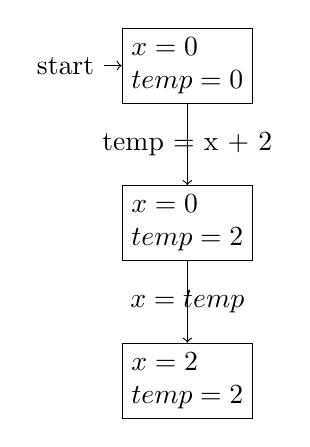
\begin{tikzpicture}[node distance=2cm, on grid, scale=0.5]
    \node[state, initial, rectangle, align=left](s1){$x=0$\\ $temp=0$};
    \node[state, rectangle, align=left, below =of s1](s2){$x=0$\\$temp=2$};
    \node[state, rectangle, align=left, below =of s2](s3){$x=2$\\$temp=2$};
    \path[->](s1) edge node {temp = x + 2}(s2);
    \path[->](s2) edge node {$x=temp$}(s3);
  \end{tikzpicture}

  \caption{State diagram of a system with a single process}
  \label{fig:sequencielstatediagram}
\end{figure}

In a sequential program with one process, there is one possibility in which order the statements are executed. Each state has only outgoing transition. When multiple processes are executed and the scheduler strategy is a priori unknown, there are several possibilities in which order the statements are executed. Interleaving is a paradigm to model systems with multiple processes. This perspective is based on the view that only one processor is available on which the statements of the programs are interlocked \cite{baier08}. In each state there is a nondeterministic choice, which process can execute the next statement. Figure \ref{fig:interleavingtransitionsystem} shows a state diagram of a system with two processes. Interleaving is an enumeration of all possible state sequences.

\subsection{Interleaving Examples}
\label{sec:interleavingexamples}

\subsubsection{Promela}
\label{sec:promela}

Spin verifies models of system behavior, written in the system specification language Promela. In the following section, concepts are explained by Promela code examples. This section is intended to contribute to the understanding of the code examples.

Promela is intended to describe abstractions of systems designs. It's specification language. A Promela model describes the behavior of a system. Promela is intended to describe concurrent software systems.

The syntax for declaration of variables is similar to the programming language C. In the following examples use the data type byte.

A keyword is defined with the keyword \verb|proctype|. \verb|proctype| is followed by the identifier of the process. The statements of the process type is enclosed in curly braces \verb|{}| \cite{holzmann03}.

The keyword \verb|active| creates a new process instance of the following process type. The process starts immediately.

\subsubsection{Sequential Programming}
\label{sec:sequential}

Listing \ref{lst:interleavingcode} shows a system with one active process. The statements are executed sequentially. An instance of the process type \verb|sequential| is created. The process reads the global variable \verb|x|, computes $x+2$ and stores the result in the variable \verb|temp|. Then \verb|temp| is assigned \verb|x|. The order of the states of the corresponding state diagram is non-ambiguous. Figure \ref{fig:sequencielstatediagram} shows the state diagram.

 \lstinputlisting[label={lst:interleavingcode},caption={system with a single process},numbers={left},float,language=Promela]{sequential.pml}  

\subsubsection{Concurrent Programming}
\label{sec:concurrent}

Listing \ref{list:interleaving2proc} shows a system with 2 active processes. The processes are executed concurrently. The processes add a constant integer to the global variable \verb|x| like the system in section \ref{sec:sequential}. There are several possibilities the computation is executed. One possible computation would first execute all statements of process \verb|A| and then all statements of process \verb|B|. The scheduler can switch the process after every transition. Figure \ref{fig:interleavingtransitionsystem} shows the interleaved state diagram of the system in listing \ref{list:interleaving2proc}.

\lstinputlisting[label={list:interleaving2proc}, caption={Add operation with 2 processes},numbers=left,float,language=Promela, ]{interleavingproc.pml}    


\begin{figure}
\centering
\scalebox{0.9}{
 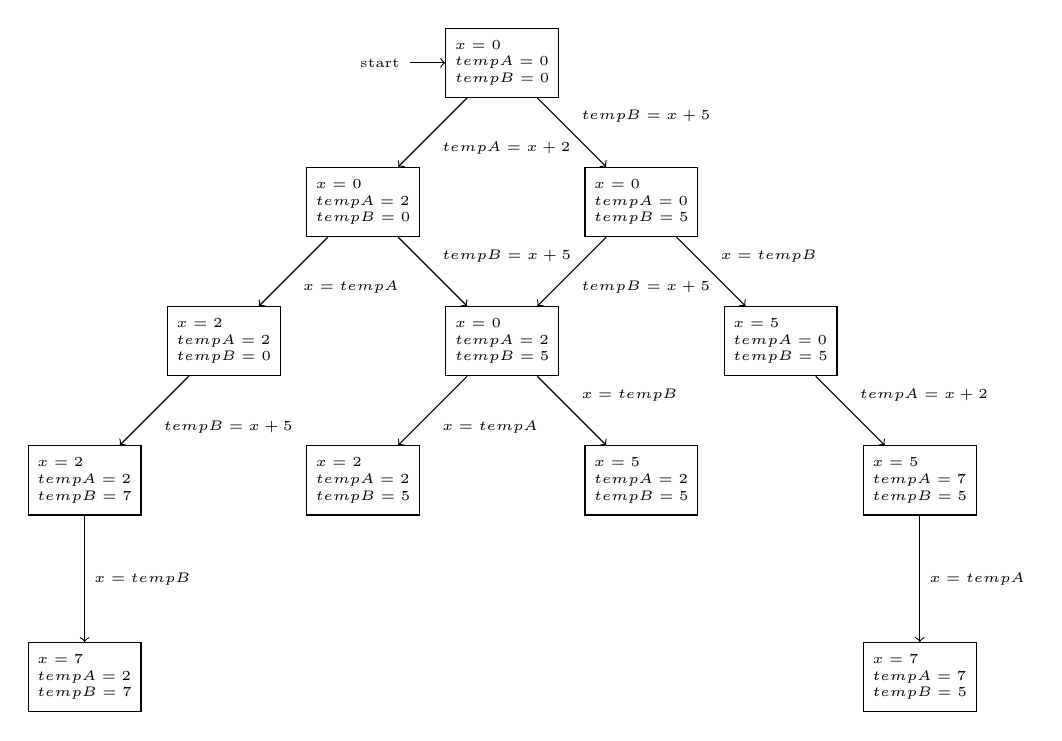
\begin{tikzpicture}[node distance=2.5cm, on grid, auto]
\tikzstyle{every node}=[font=\tiny]
   \node[state, initial, rectangle, align=left](s1){$x=0$\\$tempA=0$\\$tempB=0$};
   \node[state, rectangle, align=left](s2) [below left=of s1]{$x=0$\\$tempA=2$\\$tempB=0$};
   \node[state, rectangle, align=left](s3)[below left=of s2]{$x=2$\\$tempA=2$\\$tempB=0$};
  \node[state, rectangle, align=left](s4)[below left=of s3]{$x=2$\\$tempA=2$\\$tempB=7$};
\node[state, rectangle, align=left](s5)[below =of s4]{$x=7$\\$tempA=2$\\$tempB=7$};
\node[state, rectangle, align=left](s6)[below right=of s1]{$x=0$\\$tempA=0$\\$tempB=5$};
\node[state, rectangle, align=left](s7)[below right=of s6]{$x=5$\\$tempA=0$\\$tempB=5$};
\node[state, rectangle, align=left](s8)[below right=of s7]{$x=5$\\$tempA=7$\\$tempB=5$};
\node[state, rectangle, align=left](s9)[below =of s8]{$x=7$\\$tempA=7$\\$tempB=5$};
\node[state, rectangle, align=left](s10)[below right=of s2]{$x=0$\\$tempA=2$\\$tempB=5$};
\node[state, rectangle, align=left](s11)[below left=of s10]{$x=2$\\$tempA=2$\\$tempB=5$};
\node[state, rectangle, align=left](s12)[below right=of s10]{$x=5$\\$tempA=2$\\$tempB=5$};
   \path[->](s1) edge node {$tempA=x+2$}(s2);
   \path[->](s2) edge node {$x=tempA$}(s3);
   \path[->](s3) edge node {$tempB=x+5$}(s4);
\path[->](s4) edge node {$x=tempB$}(s5);
\path[->](s1) edge node {$tempB=x+5$}(s6);
\path[->](s6) edge node {$x=tempB$}(s7);
\path[->](s7) edge node {$tempA=x+2$}(s8);
\path[->](s8) edge node {$x=tempA$}(s9);
\path[->](s2) edge node {$tempB=x+5$}(s10);
\path[->](s6) edge node {$tempB=x+5$}(s10);
\path[->](s10) edge node {$x=tempA$}(s11);
\path[->](s10) edge node {$x=tempB$}(s12);
 \end{tikzpicture}
}
 \caption{State diagram for system in Listing \ref{list:interleaving2proc}}
\label{fig:interleavingtransitionsystem}
 \end{figure}

The state diagram \ref{fig:interleavingtransitionsystem} shows that the system from Listing \ref{list:interleaving2proc} can terminate in 4 different states. If the scheduler strategy is unknown the resulting state is non-deterministic. Model checking tools like spin are able search the state space for unwanted states. Undesirable states are defined with Linear Temporal Logic. Section \ref{sec:ltl} will explain how undesirable is defined.

\subsection{Synchronization}
\label{sec:synchronization}

Four different non-deterministic terminal states in a program that adds constant integers to a shared variable isn't normally the desired behavior. Processes can be synchronized to avoid race conditions. The following section will explain one way of synchronization on basis of an example. The example describes a synchronized variant of listing \ref{list:interleaving2proc}.

\subsection{Synchronization Examples}
\label{sec:syncexample}

Listing \ref{lst:withoutsemaphore} shows a system with two active processes with the same process type. The processes are instantiated within the \verb|init|-process. It is always the first process activated. Both processes add the value $2$ to the value stored in \verb|x|. If you like to enforce that the resulting value in \verb|x| is $4$, you have to synchronize the processes. Only one process can be in the critical section (line 4-8). This is also called mutual exclusion. One way to achieve mutual exclusion is the use of semaphores.

\lstinputlisting[label={lst:withoutsemaphore},caption={Program without mutual exclusion}, numbers=left,language=Promela]{withoutsemaphore.pml}

Listing \ref{lst:withsemaphore} shows a system that achieves mutual exclusion with semaphores. Processes have to acquire a semaphore, before they can enter the critical section. When this system terminates, the variable \verb|x| has always the value $4$.

\lstinputlisting[label={lst:withsemaphore},numbers=left,float,language=Promela,caption={Mutual exclusion with semaphores}]{semaphore.pml}

The Test \texttt{x>0} and the following \texttt{x--} operation have to be executed atomic. In Promela atomic sequences of statements are enclosed in curly braces with a preceding \texttt{atomic} keyword.

Boolean expression like \verb|x>0|, without an assignment block processes when the expression evaluates to False until it evaluates to True.

\subsubsection{Deadlock Example}
\label{sec:deadlock}

When system contains more than one lock, a deadlock may occur. Listing \ref{list:deadlock} shows a system that contains a deadlock. Given the computation of the system in which process \texttt{TakeAFirst} requests semaphore $A$ and in the next executed state process $B$ requests semaphore $B$. Both processes are waiting for the other semaphore to proceed. The system is dead.

\lstinputlisting[label=list:deadlock,numbers=left,language=Promela,caption={Synchronization with deadlock}]{deadlock.pml}

Section \ref{sec:ltl} describes how spin can detect deadlock in systems specified with Promela.

\section{Define correctness properties}
\label{sec:ltl}

The goal of model checking is to verify a behavioral model of the system against desired properties. These properties are called correctness properties. Examples for correctness properties are mutual exclusion and deadlock freedom. 

Spin read correctness properties in a formal form, called Linear Temporal Logic (LTL). This section explains correctness properties and LTL. For a better understanding of correctness properties atomic propositions and traces are described first. Atomic propositions are part of an LTL-Formula. And Traces are important because correctness properties verify traces.

\subsection{Atomic Propositions}
\label{sec:atomicpropositions}

Atomic propositions are types of declarative sentences which can either true or false. They evaluate to \verb|True| or \verb|False|. The evaluation depends on the state the system is in. The expression \verb|crit < 2| is an atomic proposition. Atomic propositions can be replaced by identifiers. For example, it is possible to define the sentence ``Process \verb|TakeAFirst| has acquired \verb|mutexA| and waits for \verb|mutexB| to be released.'' as $waitA$  that references the system in listing \ref{list:deadlock}. This example is used in section \ref{sec:safety} to describe deadlock freedom.
 
We define $AP$ as a set of atomic propositions of a system to be verified. We can map to every state a set of atomic propositions who evaluate to \verb|True|. That set of each state is a subset of $2^{AP}$.

Atomic propositions can be combined with propositional logic's operators (see table \ref{tab:operators_of_propositionallogic}.

\begin{table}[ht]
  \centering

  \begin{tabular}{l l l}
    Operator & Math & Spin \\
    not & $\neg$ & \verb|!| \\
    and & $\land$ & \verb|&&| \\
  \end{tabular}
  \caption{Operators of propositional logic }
  \label{tab:operators_of_propositionallogic}
\end{table}

\subsection{Traces and words}
\label{sec:traces}

The models that describe the behavior of a system in section \ref{sec:interleaving} can be executed in a simulation. The execution is one possible computation, a sequence of states. If the computation terminates as desired (in reactive system, computation typically do not terminate) a possible sequence starts in an initial state and ends in a defined terminal state. Every state can be mapped to a subset of $2^{AP}$. This subset contains atomic proposition that evaluate to \verb|True| in this state. A trace is a sequence of these subsets. Hence, a trace is a word over the alphabet $2^{AP}$.

A system $S$ can have multiple sequences of states. Hence, there are multiple traces in $S$. All traces of a system $S$ are referred as $Traces(S)$. $Traces(S)$ defines a language.

\subsubsection{Traceexample}
\label{sec:traceexample}

This section presents an example trace. The system that could produce the trace is shown in listing \ref{lst:criticalsection}.

\lstinputlisting[label=lst:criticalsection,caption={Critical section problem},numbers=left]{criticalsection.pml}

For a better understanding, the sequence of states is first show. A state can be represented as a triple, containing the value of the variable \verb|crit| and the locations counters of process \verb|A| and process \verb|B|. The first value shows the line number of the location counter of process \verb|A| and the second the line number of the location counter of process \verb|B|.

A possible sequence $\pi$ of states, would be:

\begin{equation}
  \label{eq:path}
  \begin{split}
\pi = (4, 9, {critA}={False},{critB}=False) \rightarrow \\
(6, 9, {critA}={True},{critB}=False) \rightarrow \\
(7, 9, {critA}={False},{critB}=False) \rightarrow \\
(7, 11, {critA}={False},{critB}=True) \rightarrow \\
(7, 12, {critA}={False},{critB}=False)
  \end{split}
\end{equation}

In this example the two Boolean variables \verb|critA| and \verb|critB| are the atomic propositions. The set of all atomic propositions in the system is

\[
\text{AP}=\{critA, critB\}
\].

The trace to the sequence of states show in equation \ref{eq:path} produces the word

\[
trace(\pi) = \varnothing \{critA\} \varnothing \{critB\} \varnothing
\].

\subsection{Linear-Time Properties}
\label{sec:satisfactionrelations}

The goal of model checking is to verify behavioral models. Verification is the evaluation of whether a system complies with a specification. So far this article dealt with the definition of the system model. To verify a system, a specification is needed. Here Linear-Time Properties come into play. Linear-time properties define which words systems can accept and which word they must not accept. A Linear-time property defines a language over the alphabet $2^{AP}$. If $S$ is the system under consideration, the language of $S$ is defined with $\text{Traces}(S)$. If $P$ is a Linear-time Property, then $S$ satisfies $P$, if $\text{Traces}(S) \subseteq P$. The Formula 
\[
TS \models P \iff \text{Traces}(S) \subseteq P 
\]
means the same. $ \models $ is a satisfaction relation\cite[p. 98]{baier08}.

Linear-time Properties can be classified into Safety-, Liveness- and Fair\-ness-Properties. The sections \ref{sec:safety} and \ref{sec:liveness} explain Safety- and Liveness-Properties.

\subsubsection{Safety-properties}
\label{sec:safety}

A safety-property verifies if a system contains undesirable states.

Deadlock freedom is a safety property. Listing \ref{list:deadlock} contains a deadlock. To verify if the system contains a deadlock a safety property can be defined as follows. Two atomic propositions are defined:
\begin{description}
\item[waitA] Process \texttt{TakeAFirst} acquired \texttt{mutexA} and waits for \texttt{mutexB}.
\item[waitB] Process \texttt{TakeBFirst} acquired \texttt{mutexB} and waits for \texttt{mutexA}.
\end{description}

Linear-time properties can be defined with a propositional logic formula. The formula for deadlock freedom for the system in listing \ref{list:deadlock} and with the given atomic propositions for one state is:
\begin{equation}
  \label{eq:pl_formula_for_deadlockfreedom}
\phi = \neg \text{waitA} \lor \neg \text{waitB}  
\end{equation}

Formula \ref{eq:pl_formula_for_deadlockfreedom} refers only to a single state in the computation. Deadlock freedom demands, that $\phi$ is true in every state of the computation. This requirement can be expressed with
\begin{equation}
  \label{eq:deadlockfreedom}
  P_{dlock} = {A_0 A_1 A_2 \dots \in (2^{AP})^{\omega} | \forall \geq i.   A_i \models \phi}
\end{equation}
. $(2^{AP})^{\omega}$ is the set of all possible words in $2^{AP}$.
Formula \ref{eq:deadlockfreedom} is a linear time property. It refers to all states in a possible computation. 

Linear time properties can also claim mutual exclusion. A safety property that demands mutual exclusion in the system $S$ of listing \ref{lst:criticalsection}, defines a language over $2^{AP}$ without the word $\{\text{critA},\text{critB}\}$. This can be formulated with
\begin{multline}
  \label{eq:mutexinwords}
  P_{mutex} = \text{set of all words} A_0 A_1 A_2 \dots \\ \text{with} \{critA,critB\} \not \subseteq A_i \text{for all } 0 \leq i
\end{multline}
or with
\begin{equation}
  \label{eq:mutex}
P_{mutex}   = {A_0 A_1 A_2 \dots \in (2^{AP})^{\omega} | \forall \geq i.   A_i \models \neg critA \lor \neg critB}
\end{equation}

A model checker verifies, if $P_{mutex}$ holds for every trace (or word) in Tra\-ces(S).

\subsubsection{Liveness-Properties}
\label{sec:liveness}

Safety properties claim, that there are no words with bad prefixes in a language. Every system S that does nothing, that is $Traces(S)=\varnothing$, satisfies every safety property. Safety properties cannot verify if progress occurs. That's where Liveness properties are needed.

Liveness properties define that every trace can be expanded so that it still holds the liveness property. A liveness property claims that an event occurs infinitely often. Liveness properties can only verify infinite traces. That means the computation of the system must not terminate.

Starvation freedom is a liveness property. Starvation freedom claims, that every waiting process eventually enters its critical section. Searching for bad prefixes cannot proof the absence of starvation freedom. A prefix only tells about the past nothing about the possible future.

\lstinputlisting[label={lst:starvation},caption={Critical section with starvation},numbers=left, language=Promela,float]{starvation.pml}

To demonstrate the definition of a liveness property listing \ref{lst:starvation} defines a system $S_{spinlock}$ that doesn't terminate and doesn't achieve starvation freedom. Process \texttt{A} tries to acquire \texttt{mutexB}. If \texttt{mutexB} isn't available it checks the availability again in an endless loop (spinlock). All traces in this system are infinite. But there are traces where process texttt{A} never reaches its critical section. This is not a desired behavior. With a liveness property it is possible to claim that there are no such traces.

The atomic proposition critA defines that the variable \texttt{critA} evaluates to True.

Starvation freedom can be defined with the liveness property
\begin{multline}
  \label{eq:starvationfreedom_in_words}
  P_{Starv} = \text{set of all infinite words } A_0 A_1 \dots A_j \in AP \\ \text{ that }\exists j \geq 0. critA \in A_j
\end{multline}
or
\begin{equation}
  \label{eq:starvationfreedom}
P_{Starv} = { A_0 A_1 \dots A_j \in (2^{AP})^{\omega} | \exists j \geq 0. critA \in A_j}
\end{equation}.
$S_{spinlock}$ doesn't satisfy $P_{Starv}$. Traces($S_{spinlock}$) contains infinite traces where critA never occurs.

\subsection{Linear Temporal Logic}
\label{sec:lineartemporallogic}

The spin model checker tool reads the system model as Promela source code. To verify the model, it needs also to read the system specification. As discussed in section \ref{sec:satisfactionrelations} with linear time properties it is possible to describe desired behavior. But it would be cumbersome to write down the linear time properties as in equation \ref{eq:starvationfreedom} for example with a keyboard. Linear Temporal Logic (LTL) is a formal logic that can express linear time properties. It can be encoded in ASCII character, so spin can read. The LTL is just one way to describe the specification of correctness properties in spin. This section report describes only the specification with LTL.

A LTL-Formula contains atomic propositions, which are connected with logic operators and with temporal operators. With temporal operators it is possible to define behavior over several states. The linear time properties in section \ref{sec:satisfactionrelations} consider all possible states. The temporal operators used in this report are shown in \ref{tab:temporal_operators}.

\begin{table}
  \centering
  \begin{tabular}{l l l}
    Operator & Math & Spin \\
    always & $\square$ & \verb|[]| \\
    eventually & $\lozenge$ & \verb|<>| \\
    implies & $\implies$ & \verb|->| \\
    until & $U$ & \verb|U|
  \end{tabular}
  \caption{Temporal operators }
  \label{tab:temporal_operators}
\end{table}

The mutual exlusion safety property $P_{mutex}$ in section \ref{sec:safety} can be formulated in LTL as follows:
\[
  {A_0 A_1 A_2 \dots \in (2^{AP})^{\omega} | \forall \geq i.   A_i \models \neg critA \lor \neg critB}
\]

\[
= \square \neg (critA,critB)
\]

The liveness property $P_{Starv}$ in section \ref{sec:liveness} can be formulated in LTL as follows:
\[
 { A_0 A_1 \dots A_j \in (2^{AP})^{\omega} \exists j \geq 0. critA \in A_j}
\]

\[
= \lozenge critA
\]

\section{Example: Traffic light system}
\label{sec:example}

This section presents an example model in Promela and verification with LTL. The example is taken from \cite{kleuker09}. In this example a simple traffic light system for a crossroads is modeled. A Traffic light has two states: green and red. The model contains only 2 instead of 4 traffic lights because opposed traffic light have always the same state. The two traffic lights are numbered with 1 and 2.

\subsection{Requirements}
\label{sec:requirements}

The following requirements are demanded
\begin{enumerate}
\item The traffic lights are either red or green
\item The traffic light switch repetitive between red and green.
\item Only one traffic light is green at a time.
\item The traffic light turn alternating to green.
\end{enumerate}

\subsection{Atomic propositions}
\label{sec:trafficlightap}

First the atomic propositions for the LTL-Formulas are defined:

\begin{description}
\item[tl1green] Traffic light 1 is green.
\item[tl1red] Traffic light 1 is red.
\item[tl2green] Traffic light 2 is green.
\item[tl2red] Traffic light 2 is red.
\item[tl1last] Traffic light 1 was green last.
\item[tl2last] Traffic light 2 was green last.
\end{description}

\subsection{LTL-Formulas}
\label{sec:exampleltl}

The requirements can be formalized as follows:

\begin{enumerate}
\item 
  \begin{multline}
    (((\text{tl1green} \lor \text{tl1red}) \land (\text{tl1green}\iff \neg \text{tl1red})) \\ \land((\text{tl2green} \lor \text{tl2red})\land (\text{tl2green} \iff \neg \text{tl2red})))
  \end{multline}
\item
  \begin{multline}
    \label{eq:ltlreq1}
    (((\text{tl1green} \implies (\lozenge \text{tl1red})) \\
    \land (\text{tlred} \implies (\lozenge \text{tl1green}))\\
    \land (\text{tl2green} \implies (\lozenge \text{tl2red})) \\
    \land (\text{tl2red} \implies (\lozenge \text{tl2green}))))
  \end{multline}
\item
  \begin{multline}
    \label{eq:ltlreq2}
    ((\text{tl1green} \implies \neg \text{tl2green}) \land (\text{tl2green} \implies \neg \text{tl1green}))
  \end{multline}
\item
  \begin{multline}
    \label{eq:ltlreq3}
    ((\text{tl1last} U(\text{tl2last} \land \neg \text{tl1last})) \\
    \land (\text{tl2last} U (\text{tl1last} \land \neg \text{tl2last}))\\
\land(\text{tl1last} \iff \neg \text{tl2last}))
  \end{multline}
\end{enumerate}

The first formula ensures that every traffic light has only two states and that the states are mutually exclusive. The second formula checks if the traffic lights switch repetitive between the states red and green. The third formula ensures that only one traffic light is green at the moment. Keep in mind that both traffic lights can be red. The fourth formula defines that traffic light have to switch. A Traffic light is red until it switches to green. It can stay green for several states until it switches back to red.

\subsection{Promela Model}
\label{sec:trafficlightsmodel}

\lstinputlisting[label={lst:trafficlightsmodel},caption={Promelamodel of the traffic light system},numbers=left,language=Promela]{trafficlights.pml}

The two traffic lights has to be synchronized. In listing \ref{lst:trafficlightsmodel} synchronization is achieved with a centralized process of type Semaphore. Processes of the process type \texttt{tafficlight} switch states their traffic light. They communicate with the semaphore process over a Promela channel in a synchronous manner. In simple terms; the semaphore process blocks or allows to pass the right process when they try to send him a p-operation message. The following paragraph explains the semantics of the listing \ref{lst:trafficlightsmodel} in detail. 

In a Promela system specification \texttt{mtype} defines symbols. They are like an enum. In listing \ref{lst:trafficlightsmodel} the symbols \texttt{p}, \texttt{v}, \texttt{red} and \texttt{green} are defined.

The state of each traffic light is represented with an array of the previously defined symbols. The array has length 2. It is defined with \texttt{mtype tlstate[]}. The system instantiates 2 processes of type trafficlight. Each process instance changes only one element of \texttt{tlstate}. The traffic light number is save in the parameter variable \texttt{name} of the proctype constructor. 
The traffic light system has a semaphore process of process type \texttt{Semaphore} that synchronizes state transmissions.  The trafficlight processes communicate with the semaphore process over the channel \texttt{center}. A channel is defined with the keyword \texttt{chan}. \texttt{chan center=[0] of \{mtype,bit\}} defines a channel that accepts pair of values with the type \texttt{mtype} and \texttt{bit}. It's a synchronous channel.  \texttt{center!p,name;} is the p-operation. A traffic light tries to send the semaphore process the value pair of the p-symbol and its number as bit. \texttt{center!p,name;} block until the semaphore process read the channel with \verb|center?p,eval(next_tl);|. \texttt{eval} is needed because the \texttt{center?}-statement can contain values and variables. Values are matched against the incoming values. If the statement contains a variable, the incoming value is stored in that variable. In this example the first behavior is desired. Reading means that the values must match. The semaphore process waits for an incoming p symbol and the number of the traffic light who is next green. The semaphore process controls this way which traffic light is green next. If the semaphore process accepts the message from the trafficlight process, the trafficlight process can proceed and change it's tlstate element first to green and then to red. Afterwards it sends a v-operation message with \texttt{center!v,name;}. This message is always accepted by the semaphore process with \verb|center?v,_;|. \verb|_| is a global variable. The value is saved there but never used. After the semaphore process received the v-operation it changes the variable \verb|next_tl| to the other traffic light number.


\begin{lstlisting}[label={lst:spinltl},caption={LTL-properties with formalized atomic propositions for spin}]
#define tl1red(tlstate[0]==red)
#define tl1green(tlstate[0]==green)
#define tl2red (zustand[1]==rot)
#define tl2green (zustand[1]==gruen)
#define tl1last (next_tl==1)
#define tl2last (next_tl==0)

/* 1. */
[] ( ( (tl1red || tl1green)
&&(tl1red <-> (!tl1green)))
&&( (tl2red || tl2green)
&&(tl2red <-> (!tl2green))) )
/* 2 */
[] ( (tl1red -> (<> tl1green))
&&(tl1green -> (<> tl1red))
&&(tl2red -> (<> tl2green))
&&(tl2green -> (<> tl2red)) )
/* 3 */
[] ( (tl1green -> (!tl2green))
&&(tl2green -> (!tl1green)) )
/* 4 */
[] ( (tl1last
U (tl2last && (!tl1last)))
&&(tl2last
U (tl1last && (!tl2last)))
&& (tl1last <-> (!tl2last)) )
\end{lstlisting}

In listing \ref{lst:spinltl} the atomic propositions of \ref{sec:exampleltl} are formalized and defined as macros. Spin can test the LTL-Formulas from listing \ref{lst:spinltl} hold in the model of listing \ref{lst:trafficlightsmodel}.

\begin{thebibliography}{9}
\bibitem{baier08}
Christel Baier Joost-Pieter Katoen,
Principles of Model Checking,
The MIT Press,
2008.

\bibitem{holzmann03}
Gerald Holzmann,
The Spin Model Checker: Primer and Reference Manual,
Addison-Wesley Professional,
2003.

\bibitem{kleuker09}
Stephan Kleuker,
Formale Modelle der Softwareent\-wicklung,
View\-eg+\-Teub\-ner,
2009.

\end{thebibliography}

\end{document}

%%% Local Variables: 
%%% mode: latex
%%% TeX-master: "master"
%%% End: 
